
In this section we assume that the points are in 2D and come in a random order. In particular, for all sets of points $P$, every permutation of $P$ must have equal probability density.
\\

A special case of this is if the data points are generated from independent identical distributions. In this case, the probability density of a particular ordered point stream $P$ occuring can be factored into the product of the probability densities of each individual point occuring. Since multiplications can be reordered, this total probability is independent of the order in which the points occur.
\\

What makes the model powerful is that we are not making any assumptions about the distribution from which each individual point is generated, but simply that they are i.i.d. So this assumption would hold if the data points were generated from a mixture model, LDA, or even generalizations of these.
\\

\section{Algorithm Description}

Recall the definition of an interior point.

\begin{definition}
We say a point $p$ is interior to $P$ if $p$ is in the convex hull of $P \setminus \{p\}$.
\end{definition}

Our algorithm is simple. We begin by keeping a set $S = \{\}$. For each point $p \in P$ that the algorithm sees, if the distance from $p$ to the convex hull of $S$ is at most $\epsilon$, we discard $p$. Otherwise, we add $p$ to $S$. This is illustrated in figure 1: if the point $p$ is inside (figure~\ref{fig:point_inside_hull}) or near $S$ (figure~\ref{fig:point_slightly_outside_hull}) we discard $p$. Otherwise (figure~\ref{fig:point_far_outside_hull}) we add $p$ to $S$.
\\

\begin{figure}[!htb]
\centering
\begin{subfigure}[b]{.33\linewidth}
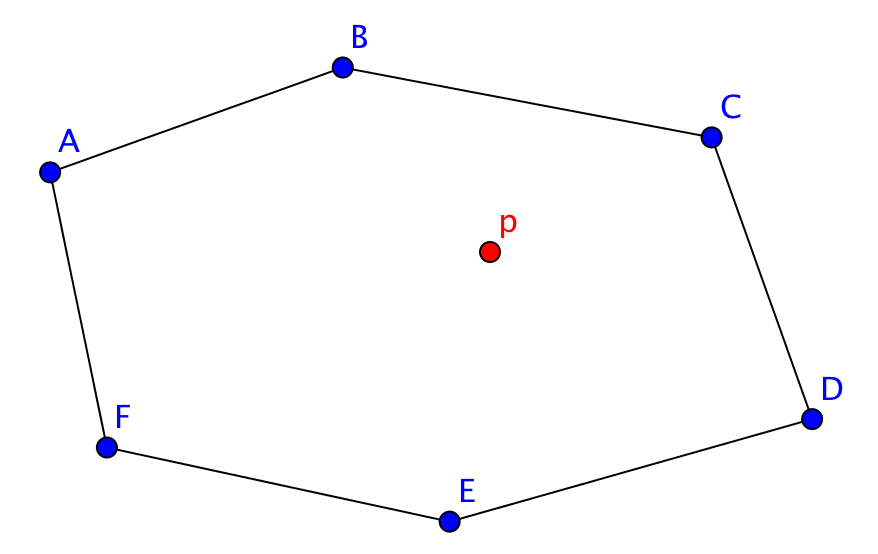
\includegraphics[width=\linewidth]{point_inside_hull}
\caption{Discard: $p$ inside hull}\label{fig:point_inside_hull}
\end{subfigure}\hspace{20 mm}
\begin{subfigure}[b]{.33\linewidth}
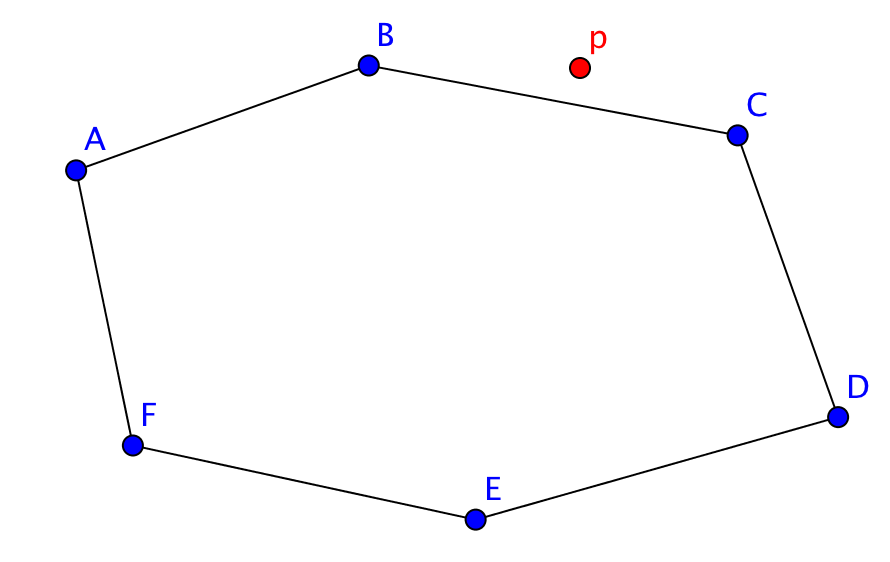
\includegraphics[width=\linewidth]{point_slightly_outside_hull}
\caption{Discard: $p$ near hull}\label{fig:point_slightly_outside_hull}
\end{subfigure}\hspace{20 mm}
\begin{subfigure}[b]{.33\linewidth}
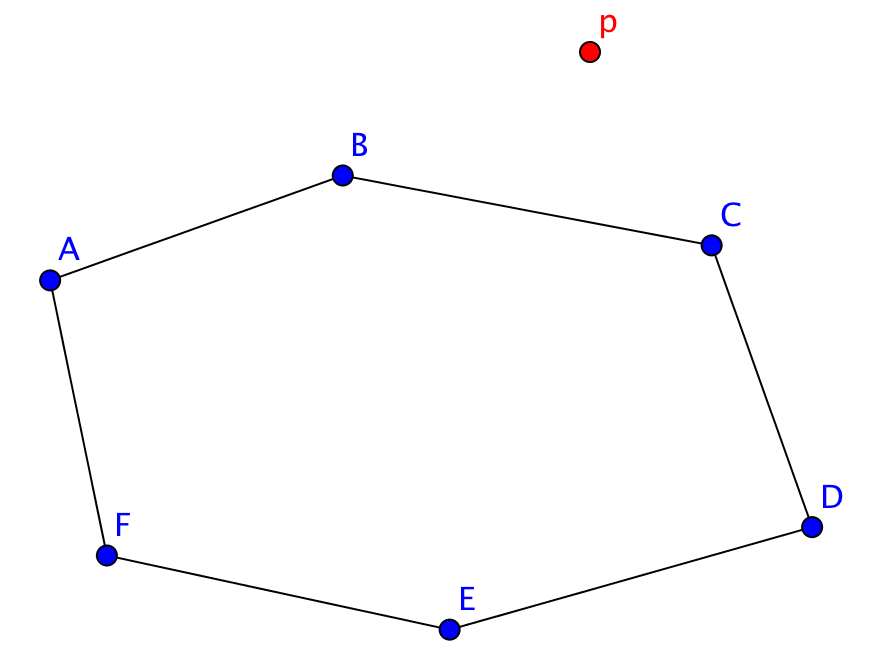
\includegraphics[width=\linewidth]{point_far_outside_hull}
\caption{Keep: $p$ far from hull}\label{fig:point_far_outside_hull}
\end{subfigure}
\caption{Our algorithm keeps point $p$ only if it is far from the current hull.}
\label{fig:when_to_discard_random_order}
\end{figure}

We then repeatedly delete interior points in $S$ until $S$ has no interior points. Figure~\ref{fig:2_interior_points} shows a point set with 2 interior points, and figure~\ref{fig:no_interior_points} shows the point set after removing all the interior points.
\\

\begin{figure}[!htb]
\centering
\begin{subfigure}[b]{.33\linewidth}
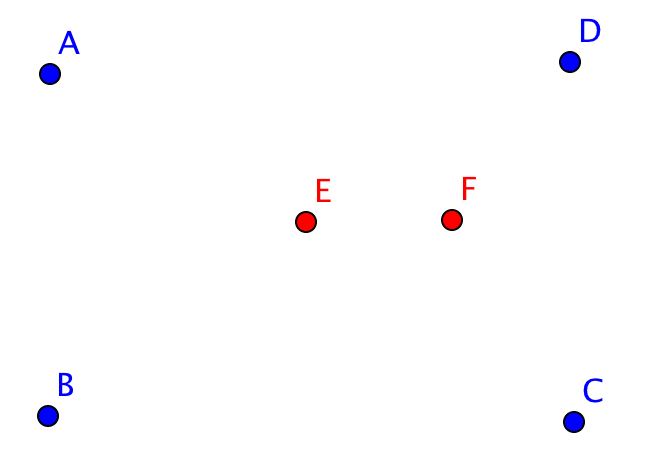
\includegraphics[width=\linewidth]{2_interior_points}
\caption{Interior points in red}\label{fig:2_interior_points}
\end{subfigure}\hspace{20 mm}
\begin{subfigure}[b]{.33\linewidth}
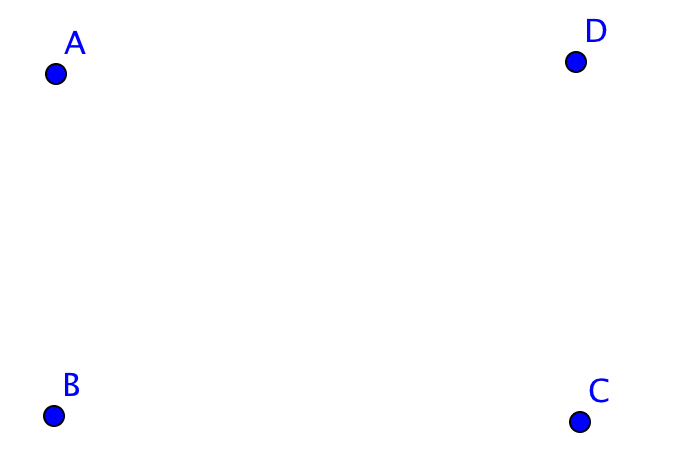
\includegraphics[width=\linewidth]{no_interior_points}
\caption{No interior points}\label{fig:no_interior_points}
\end{subfigure}
\caption{Our algorithm iteratively removes interior points from $S$.}
\label{fig:interior_points}
\end{figure}

The algorithm, which we call ROA, is summarized below.
\\

\begin{figure}
\begin{lstlisting}[escapechar=|]
S = {}
for p |$\in$| P:
  if dist(p, S) |$\leq$| |$\epsilon$|:
    // Discard p
  else:
    S = S |$\cup$| {p}
    while S has an interior point p:
      Delete p from S
\end{lstlisting}
\caption{Pseudocode for random order algorithm.}
\end{figure}

\section{Proof Outline}

\begin{theorem}
(Correctness) After processing point stream $P$, ROA keeps an $\epsilon$-approximate convex hull $S$ of $P$.
\end{theorem}

\begin{proof}
Let $S_i$ be $S$ after the $i^{\mbox{th}}$ iteration of the `for' loop on line 2. We show by induction that $S_i$ is an $\epsilon$-approximate convex hull of the first $i$ points in $P$. The base case for $i = 0$, $S_0 = \{\}$ holds because $\{\}$ is an $\epsilon$-approximate convex hull of $\{\}$.
\\

For the inductive step, suppose that $S_i$ is an $\epsilon$-approximate convex hull of the first $i$ points in $P$. Because we only remove interior points in $S$, the convex closure of $S_{i+1}$ contains the convex closure of $S_i$. This means that $S_{i+1}$ is an $\epsilon$-approximate convex hull of the first $i$ points in $P$. Furthermore, we keep the $(i+1)^{\mbox{th}}$ point $p$ iff dist$(p, S) > \epsilon$. This ensures that $p$ is within distance $\epsilon$ from $S_{i+1}$.
\end{proof}

We use 2 simple results in our 2D proof, that we sketch out for completeness.

\begin{lemma}
(1D Space) Suppose we run ROA on $P \subseteq \mathbb{R}$. After processing $P$, ROA keeps at most 2 points in $S$.
\end{lemma}

\begin{proof}
$S$ will contain the minimum and maximum point.
\end{proof}

\begin{lemma}
(1D Insertion Only Space) Suppose we run ROA, except we do not run lines 7 and 8, which involve deleting interior points from $S$. In other words, the size of $S$ is non-decreasing. Then there exists $m$, s.t. for all point streams $P \subseteq \mathbb{R}$ containing $n$ points, with probability at least $1 - 1/n^3$ ROA keeps at most $m(1 + \log{n})$ points in $S$. In other words, with high probability, the size of $S$ is $O(\log{n})$.
\end{lemma}

\begin{proof}
We order the points/numbers in increasing order. We might have multiple copies of the same point, in which case we break ties in our ordering arbitrarily. This means that if $a$ and $b$ are points in stream $P$ at indices $i$ and $j$ with $i \neq j$, then $a < b$ or $a > b$ in our ordering, even if $a$ and $b$ are the same real number in $\mathbb{R}$.
\\

Consider the first $i$ points received. By the random order assumption, all permutations of the first $i$ points are equally likely. We only keep the $i^{\mbox{th}}$ point if it is strictly less than, or strictly greater than, the first $i-1$ points received. Because of the special ordering we constructed, this happens with probability $2/i$ (except when $i = 1$ in which case it is 1) and is independent for each $i$. 
\\

By an integral bound, we can show that,
\[ 1 + \sum_{i=1}^n \frac{2}{i} \leq 2\log{n} + 1 \]
Then, applying a Chernoff bound we get the desired result.
\end{proof}

We will, perhaps surprisingly, reduce the 2D case to the 1D insertion only case.

\begin{theorem}
\label{thm:2droaspace}
(2D Space) There exists $m \in \mathbb{R}$, such that for all point streams $P \subseteq \mathbb{R}^2$ containing $n$ points, with probability at least $1 - 1/n^2$, ROA keeps at most $m\mbox{OPT}(P, \epsilon)(1 + \log{n})$ points in $S$. In other words, with high probability, the size of $S$ is $O(\mbox{OPT}(P, \epsilon)\log{n})$.
\end{theorem}

\begin{proof}
Consider an optimal $\epsilon$-approximate convex hull (of $P$) $O$. Let $A$ be the set of all points in $\mathbb{R}^2$ that are contained inside the convex closure of $O$, but within distance $\epsilon$ of the boundary of the convex closure of $O$. We call $A$ the ``inner" set of $O$. Let $B$ be the set of all points in $\mathbb{R}^2$ that are outside of the convex closure of $O$, but within distance $\epsilon$ of the boundary of the convex closure of $O$. Let the ``deep interior" be all points in $\mathbb{R}^2$ that are inside the convex closure of $O$ but not in the ``inner" set $A$.
\\

For example, in figure 1(a), the convex closure of $O$ defines a rectangular region. The original set of points $P$ is not shown. $A$ is the region shaded in green in figure 1(b). Intuitively, all points that are inside the rectangular region defined by $O$, but not too far inside, are in $A$. In figure 1(b) we also marked the deep interior, the set of points contained in $O$ but not in $A$. $B$ is the region shaded in blue in figure 1(c).  Intuitively, all points that are outside the rectangular region defined by $O$, but not too far outside, are in $B$.
\\

\begin{figure}[!htb]
\centering
\begin{subfigure}[b]{.4\linewidth}
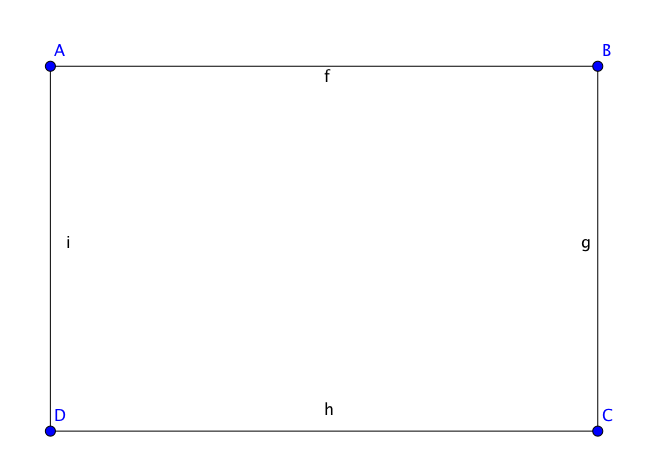
\includegraphics[width=\linewidth]{original_shape}
\caption{Original shape}\label{fig:mouse}
\end{subfigure}\hspace{20 mm}
\begin{subfigure}[b]{.4\linewidth}
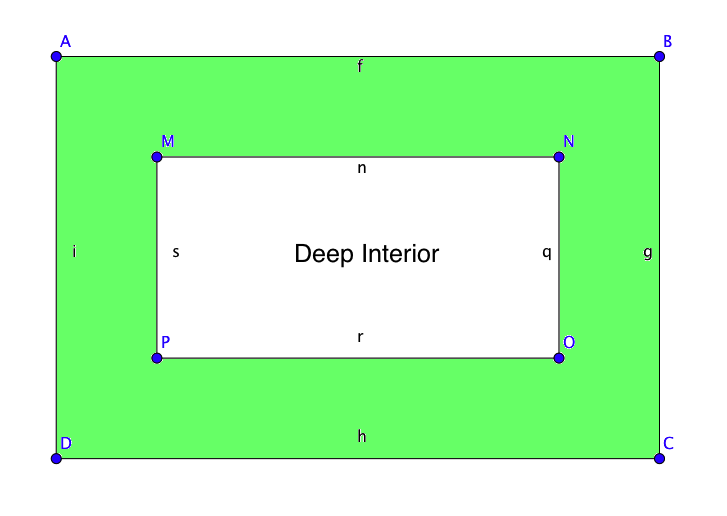
\includegraphics[width=\linewidth]{inner_boundary}
\caption{Inner set $A$ in green}\label{fig:gull}
\end{subfigure}

\begin{subfigure}[b]{.4\linewidth}
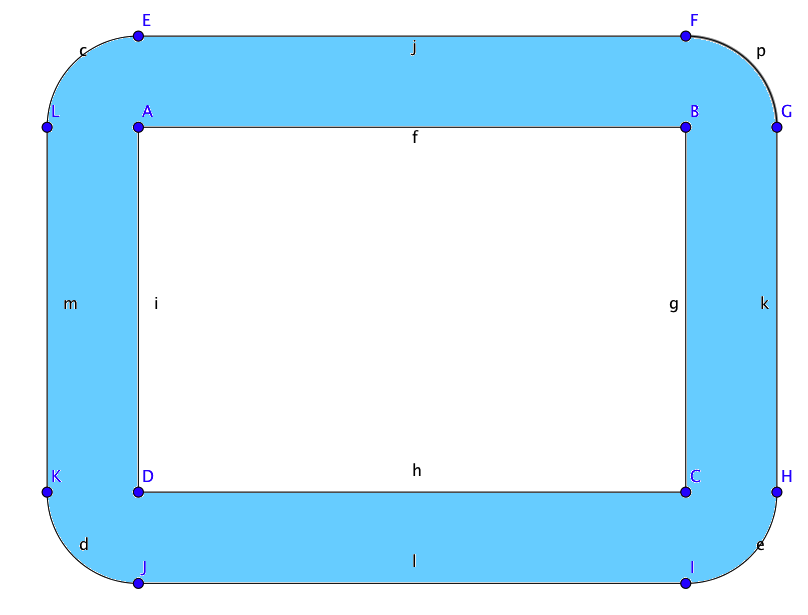
\includegraphics[width=\linewidth]{outer_boundary}
\caption{Outer set $B$ in blue}\label{fig:tiger}
\end{subfigure}\hspace{20 mm}
\caption{Illustration of inner and outer sets for approximate convex hull}
\label{fig:animals}
\end{figure}

\begin{lemma}
The boundary $U$ of the convex closure of $S$ must be contained in the union of $A$ and $B$.
\label{lem:sboundary}
\end{lemma}

\begin{proof}
First, we show that $U$ cannot intersect with the deep interior. To see this, suppose we choose the origin to be contained inside the deep interior (if the deep interior is empty then the claim is vacuously true). $S$ is an $\epsilon$-approximate convex hull of $P$ and $O \subseteq P$, so $S$ is an $\epsilon$-approximate convex hull of $O$. Then for all unit vectors $v$, |$\max_{o \in O} \langle o, v \rangle$ - $\max_{s \in S} \langle s, v \rangle| \leq \epsilon$. That is, in every direction, $U$ must be within distance $\epsilon$ from the boundary of the convex closure of $O$. But in every direction, the deep interior is greater than distance $\epsilon$ from the boundary of the convex closure of $O$.
\\

Next, we need to show that all points in the convex closure of $S$ are within distance $\epsilon$ from the convex closure of $O$. But this is true because $O$ is an $\epsilon$-approximate convex hull of $P$ and $S \subseteq P$, so $O$ is an $\epsilon$-approximate convex hull of $S$.
\end{proof}

By lemma~\ref{lem:sboundary}, since we delete all interior points in $S$ (lines 7 and 8), every point in the deep interior will be eventually discarded. Now, examine figure 2, which shows the top half of the original rectangle defined by $O$, along with corresponding parts of $A$ and $B$. Regions $C1, C2, E$ are part of the outer set $B$, and $I$ is part of the inner set $A$. In regions $C1$ and $C2$ we will select at most a constant number of points, because it is contained in a circle of radius $\epsilon$. There are OPT such regions. 
\\

In region $E$, we can use an argument similar to the 1D case to show that we will select, with high probability, at most $O(\log{n})$ points. This is because the height of $E$ is $\epsilon$. The idea is that we can view the line $AB$ as the $x$-axis, and consider the $x$-coordinate of each point in $O$. We will discard every new point in $E$ unless it has $x$-coordinate greater than all the current points we have seen in $E$, or $x$-coordinate lesser than all the current points we have seen in $E$. This reduces the problem to the 1D insertion only problem, so with probability $1-1/n^3$ we keep $O(\log{n})$ points.
\\

\begin{figure}
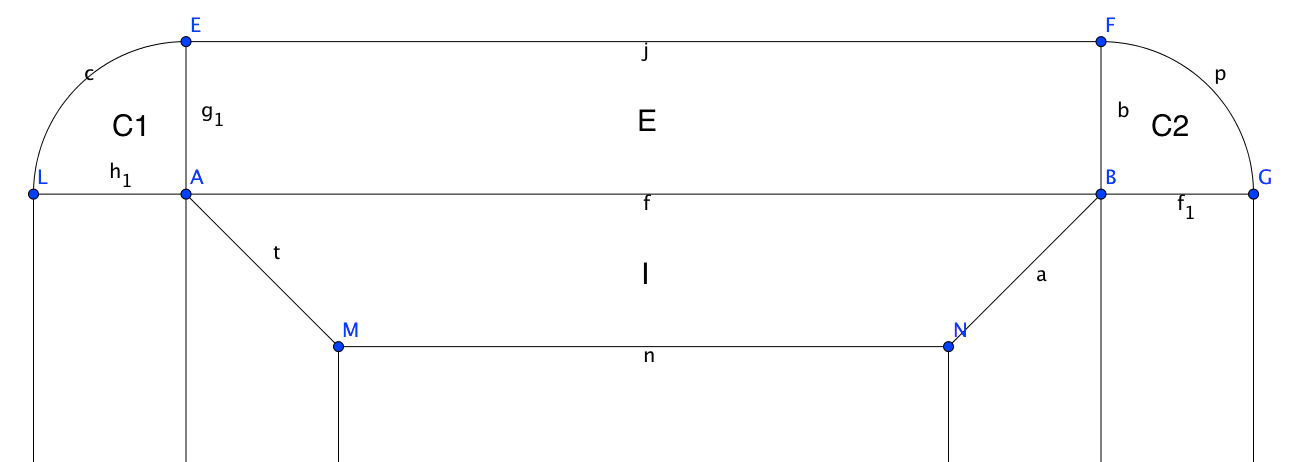
\includegraphics[width=\linewidth]{main_regions}
\caption{Important regions around approximate convex hull}\label{fig:tiger}
\end{figure}

The same argument applies to $I$. Note that there are OPT regions like $I$ and OPT regions like $E$, so by union bound, the total number of points we keep is $O(\mbox{OPT} \cdot \log{n})$ with high probability.
\end{proof}

Note that theorem~\ref{thm:2droaspace} gives us a high probability bound so:
\begin{enumerate}
\item Since ROA never keeps more than $n$ points (the entire set), we can use the high probability bound to show that the expected number of points ROA keeps is $O(\mbox{OPT}\log{n})$.
\item We can show that with high probability, when ROA has processed a prefix $P'$ containing the first $i$ out of $n$ points of $P$, ROA keeps an $\epsilon$-approximate convex hull of size $O(\mbox{OPT}(P', \epsilon)\log{n})$. Importantly, with high probability, this holds \emph{for all prefixes}, that is, throughout the entire stream.
\end{enumerate}

Unfortunately, this algorithm does not give good gaurantees in 3D. The 3D case reduces to the 2D intertion only case, where we run ROA without removing interior points. However, in the worst case we might end up choosing a large number of points.
